%% GABARIT POUR THÈSE PAR ARTICLES
%%
%% Consulter la documentation de la classe ulthese pour une
%% description détaillée de la classe, de ce gabarit et des options
%% disponibles.
%%
%% [Ne pas hésiter à supprimer les commentaires après les avoir lus.]
%%
%% Déclaration de la classe avec le type de grade
%%   [l'un de LLD, DMus, DPsy, DThP, PhD]
%% et les langues les plus courantes. Le français sera la langue par
%% défaut du document. L'option 'bibsection' permet de créer des
%% bibliographies par chapitre présentées sous forme de section
%% numérotée.
\documentclass[PhD,bibsection,english,french]{ulthese}
  %% Encodage utilisé pour les caractères accentués dans les fichiers
  %% source du document. Les gabarits sont encodés en UTF-8. Inutile
  %% avec XeLaTeX, qui gère Unicode nativement.
  \ifxetex\else \usepackage[utf8]{inputenc} \fi

  %% Charger ici les autres paquetages nécessaires pour le document.
  %% Quelques exemples; décommenter au besoin.
  %\usepackage{amsmath}       % recommandé pour les mathématiques
  %\usepackage{ncccomma}      % gestion de la virgule dans les nombres

  %% Utilisation d'une autre police de caractères pour le document.
  %% - Sous LaTeX
  %\usepackage{mathpazo}      % texte et mathématiques en Palatino
  %\usepackage{mathptmx}      % texte et mathématiques en Times
  %% - Sous XeLaTeX
  %\setmainfont{TeX Gyre Pagella}      % texte en Pagella (Palatino)
  %\setmathfont{TeX Gyre Pagella Math} % mathématiques en Pagella (Palatino)
  %\setmainfont{TeX Gyre Termes}       % texte en Termes (Times)
  %\setmathfont{TeX Gyre Termes Math}  % mathématiques en Termes (Times)

  %% Gestion des hyperliens dans le document. S'assurer que hyperref
  %% est le dernier paquetage chargé.
  \usepackage{hyperref}
  \hypersetup{colorlinks,allcolors=ULlinkcolor}

  %% Options de mise en forme du mode français de babel. Consulter la
  %% documentation du paquetage babel pour les options disponibles.
  %% Désactiver (effacer ou mettre en commentaire) si l'option
  %% 'nobabel' est spécifiée au chargement de la classe.
  \frenchbsetup{%
    StandardItemizeEnv=true,       % format standard des listes
    ThinSpaceInFrenchNumbers=true, % espace fine dans les nombres
    og=«, fg=»                     % caractères « et » sont les guillemets
  }

  %% Suppression du numéro de section de la bibliographie. Utilisation
  %% de \extrasfrench parce que c'est la dernière langue déclarée dans
  %% \documentclass, ci-dessus.
  %\addto\extrasfrench{%
  %  \renewcommand{\bibsection}{\section*{\bibname}\prebibhook}}

  %% Déclarations des pages de titre. Remplacer les éléments entre < >.
  %% Supprimer les caractères < >. Couper un long titre ou un long
  %% sous-titre manuellement avec \\.
  \titre{<Titre principal>}
  % \titre{Ceci est un exemple de long titre \\
  %   avec saut de ligne manuel}
  % \soustitre{Sous-titre le cas échéant}
  % \soustitre{Ceci est un exemple de long sous-titre \\
  %   avec saut de ligne manuel}
  \auteur{Gwenaëlle Lemoine}
  \annee{<2020>}
  \direction{Arnaud Droit, directeur de recherche}
  % \codirection{<Prénom Nom>, <codirecteur ou codirectrice> de recherche}
  % \codirection{<Prénom Nom>, <codirecteur ou codirectrice> de recherche \\
  %              <Prénom Nom>, <codirecteur ou codirectrice> de recherche}

\begin{document}

\frontmatter                    % pages liminaires

\pagestitre                     % production des pages de titre

\chapter*{Résumé}                      % ne pas numéroter
\phantomsection\addcontentsline{toc}{chapter}{Résumé} % inclure dans TdM

\begin{otherlanguage*}{french}
L'analyse par réseau de co-expression de gènes est un outil entré il y a 15 ans dans l'ensemble des outils disponibles pour l'analyse transcriptomique. En étudiant la variation de synchronisation de l'expression des gènes, cet outil permet de révéler de nouveaux gènes impliqués dans des maladies ou phénotypes dont l'expression seule n'est pas significativement différente. Il est également capable de détecter des groupes de gènes, ou modules, interagissant préférentiellement et sur lesquels il est possible d'effectuer une exploration étendue. Il est ainsi possible d'utiliser des méthodes avec injection de connaissance préalable comme l'enrichissement de gènes ou l'association phénotypique, ou des méthodes guidées par les données comme l'analyse topologique ou la co-expression différentielle. Pourtant, ce type d'analyse reste sous exploitée actuellement par rapport à son potentiel, et notamment dans certaines maladies ou phénotypes où l'altération est une désorganisation du système comme le vieillissement. 

Afin de faciliter à tout chercheur l'emploi de cette méthode, un progiciel R disponible sur Bioconductor et nommé GWENA a été développé. Organisé comme un pipeline d'analyse simplifié et allant de la construction du réseau jusqu'à l'aide à l'interprétation des modules entre différentes conditions, c'est également le seul pipeline actuel à intégrer la co-expression différentielle. Pour assister l'utilisateur, il comprend de nombreux avertissements sur l'intégrité des données rentrées et sur la plausibilité des résultats. Afin de limiter le recours à d'autres logiciels, il contient également un système de visualisation des réseaux. Enfin, GWENA est un outil dont l'architecture modulaire lui permettra d'évoluer avec le temps.

L'efficacité de GWENA a été démontrée dans une première étude du vieillissement du muscle squelettique humain où un sous ensemble de gènes a été priorisé pour l'étude de la sarcopénie. Il a également permis de préciser une topologie du réseau spécifique du vieillissement et observée auparavant : la perte de connectivité du réseau, ou déconnexion. En effet, parallèlement à la déconnexion, il a été constaté grâce à GWENA une reconnexion locale située au niveau des gènes pivots. Pour étudier cette topologie à large échelle, l'analyse a été répétée sur un ensemble élargi de tissus humains. Par un recoupement des modules différentiellement exprimés, des phénomènes communs du vieillissement entre tissus sont apparus ainsi que des phénomènes spécifiques à certains tissus. L'analyse topologique, notamment de la déconnexion, des gènes inclus dans ces recoupements pour deux exemples, un phénomène commun et un phénomène spécifique, a à son tour permis la priorisation de gènes encore mal étudiés ou inconnus dans ces phénomènes.

En finalité, les travaux présentés au cours de cette thèse auront amené à la création d'un outil utile à la communauté de biologistes comme bio-informaticiens pour faciliter l'accès à une analyse à a haut potentiel dans l'analyse du vieillissement et toute autre condition, notamment celles axées sur la dérégulation de l'expression systémique.

\textbf{Mots-clefs :} co-expression, réseau, vieillissement, transcriptomique, progiciel R, Bioconductor, co-expression différentielle.
\end{otherlanguage*}
                % résumé français
\chapter*{Abstract}                      % ne pas numéroter
\phantomsection\addcontentsline{toc}{chapter}{Abstract} % inclure dans TdM

\begin{otherlanguage*}{english}
  Text of English abstract.
\end{otherlanguage*}
              % résumé anglais
\cleardoublepage

\tableofcontents                % production de la TdM
\cleardoublepage

\listoftables                   % production de la liste des tableaux
\cleardoublepage

\listoffigures                  % production de la liste des figures
\cleardoublepage

\dedicace{Dédicace si désiré}
\cleardoublepage

\epigraphe{Texte de l'épigraphe}{Source ou auteur}
\cleardoublepage

\chapter*{Remerciements}         % ne pas numéroter
\phantomsection\addcontentsline{toc}{chapter}{Remerciements} % inclure dans TdM

Je remercie mon directeur, le Dr. Arnaud Droit, pour m'avoir accueillie dans son laboratoire.

Merci également aux membres du jury, la Dre. Francine Durocher, le Dr. Simon Hardy, le Dr. Yoann Bossé, la Dre. Sarah Gagliano Taliun, pour avoir accepté de siéger et évaluer mes travaux.

Enfin, merci à tous mes proches qui m'ont accompagnée durant ces années.
         % remerciements
\chapter*{Avant-propos}         % ne pas numéroter
\phantomsection\addcontentsline{toc}{chapter}{Avant-propos} % inclure dans TdM

% L’avant-propos contient les renseignements sur:
% - l’état de publication des articles intégrés (dates de soumission, d'acceptation ou de publication)
% - les modifications entre la version intégrée de l’article et sa version publiée, s’il y a lieu 
% - votre statut d’auteur (principal ou non)
% - votre rôle exact dans la préparation de chaque article
% - les coauteurs de chaque article

\section{Projets principaux}

Cette thèse est réalisée avec l'insertion d’articles écrits durant mon doctorat. Elle présente l’état de mes travaux dont le but principal était le développement d’outils et méthodes pour la détection de gènes candidats au vieillissement humain par l'utilisation de réseaux de co-expression de gènes. Chaque chapitre est donc constitué d'un article publié ou visant à l'être.

Les articles insérés sont les suivants :
\begin{itemize}
    \item \textit{GWENA: gene co-expression networks analysis and extended modules characterization in a single Bioconductor package}, publié dans la revue \textit{BMC Bioinformatics} le 25 mai 2021.
    \item \textit{Analyse trans-tissus par réseau de co-expression de gènes pour la détection de fonctions physiologiques communes et spécifiques au vieillissement}, article à traduire et soumettre dans la revue PLoS One.
\end{itemize}


\section{Contribution à l'article "GWENA"}

Je suis responsable de la conception, développement et maintenance de l'outil GWENA ainsi que de l'écriture de l'article. D'un point de vue analyse pour le cas d'utilisation, je suis responsable du traitement des données ainsi que de leur analyse. Le choix de la méthodologie fut un travail conjoint de Marie Pier Scott-Boyer qui a également supervisé le projet. Elle a également avec Olivier Périn, Bathilde Ambroise et Arnaud Droit participé à la relecture de l'article. L'intégralité de l'article a été validé par tous les auteurs. Arnaud Droit s'est également chargé de la recherche de financement.


\section{Contribution à l'article d'analyse trans-tissus du vieillissement via GWENA}

Je suis responsable de la conception du projet, du traitement et de l'analyse des données, de l'interprétation des résultats, et de la rédaction de l'article. Marie Pier Scott-Boyer a assisté dans la consolidation de la méthodologie et sa validation. Arnaud Droit s'est chargé de la recherche de financement.


\section{Projets annexes}

Durant mon doctorat, j'ai également pu m'investir dans différents projets scientifiques :
\begin{itemize}
    \item \textit{Weighted gene co-expression network analysis identifies inflammaging biomarkers in aged skin of humans in vivo}. Projet de ré-analyse des données de transcriptomique de Kuehne et al. 2017 par le biais de GWENA. Il a permis de mettre en évidence des gènes impliqués dans le phénomène d'inflammation chronique de faible intensité dans des biopsies d'épiderme. Par respect envers la clause de confidentialité de la chaire de recherche et d'innovation L'Oréal en biologie numérique, ces travaux n'ont pas été soumis à publication.
    \item Étude à travers de multiples points temporels sur 28 jours de la reconstruction épidermique basée sur un modèle d'épiderme \textit{in vitro} provenant de biopsies de circoncisions. Travaux effectués pour la chaire de recherche et d'innovation L'Oréal en biologie numérique et confidentiels.
\end{itemize}


\todo[inline]{Si projets non doctoraux ajoutés en annexe (ACCEM, illustration scientifique, bioinfo-fr.net, mette cette phrase : D'autre travaux scientifiques non académiques ont également été réalisés et sont visibles en Annexe \\ref{}}


\section{Financements}

Les travaux présentés dans cette thèse ont étés soutenus par la Chaire de recherche et d'innovation L'Oréal en biologie numérique.

\section{Notes}

\begin{itemize}
    \item L'intégralité des figures a été réalisée par mes soins et est sous licence CC-BY-NC sauf mention contraire ou citation d'une figure d'une publication.
    \item L'article situé en Chapitre \ref{chapter:gwena} est publié dans BMC Bioinformatics sous la licence CC-BY
    \item Pour plus d'information sur les licences Creative Commons : \url{https://creativecommons.org/about/cclicenses/}
\end{itemize}           % avant-propos

\mainmatter                     % corps du document

%%%%%%%%%%%%%%%%%%
%% INTRODUCTION %%
%%%%%%%%%%%%%%%%%%

\setcounter{chapter}{1}         % permet de débuter l'intro à 1. au lieu de 0.
\chapter*{Introduction}         % enlève la numérotation
\phantomsection\addcontentsline{toc}{chapter}{Introduction} % inclus l'intro dans la table des matières
\graphicspath{ {./img/intro} }

%% ######################
%% GROSSE AIDE A LA BIBLIO https://www.connectedpapers.com
%% #####################




%%%%%%%%%%%%%%%%%% LA COMPLEXITÉ DU VIVANT %%%%%%%%%%%%%%%%%%

\section{La complexité du vivant}

\subsection{D'un code unique à un fonctionnement multiple}

Bien que toutes les cellules d'un organisme possèdent la même information génétique via un ADN identique, plusieurs types cellulaires de fonction différente cohabitent pour former des tissus variés. Ces différences provennant d'un contrôle de l'expression ou de la répréssion d'un gène sont le fruit d'un ensemble de mécanismes de régulation établis dès les premières différenciations cellulaire dans le développement d'un organisme. Différentes types de mécanismes vont alors impacter la qualité et la quantité d'ARN messager (ARNm) produit par les cellules :
\begin{itemize}
\item La régulation de l'initiation de la transcription : la fixation d'une protéine sur l'ADN entraine l'impossibilité de fixation de l'ARN polymérase ou à l'inverse favorise son recrutement pour la transcription d'un gène.
\item  La conformation de la chromatine : les repliements de l'ADN pour la condenser dans une cellule implique de rendre disponible certaines régions à la transcription et indisponible d'autres.
\item La modification post transciptionnelle : les ARNm nécessitent l'ajout d'une 7-methylguanosine sur l'extrémité 5' (coiffe 5'), un épissage alternatif, et une polyadenylation (queue poly A) sur l'extrémité 3' afin d'être traduits en protéine. En leur absence, ces ARNm sont détruits par la cellule.
\item  La méthylation : les îlots CpG situés sur l'ADN (notamment dans les promoteurs) peuvent subir l'ajout d'un groupement méthyl, empêchant alors la fixation de différents agents de la transcription.
\item La susceptibilité à la dégradation : afin de perdurer plus de quelques minutes dans la cellule [\^Yu\_2001], certains ARN contiennent ou évitent certains motifs de nucléotides (éléments riches en AU, codon stop prématuré, taille de queue poly-A) ou bien sont victimes d'ARN non codants (ARNmi et ARNip) qui vont favoriser leur dégradation
% \item [^Yu_2001]: Yu J, Russell JE. Structural and functional analysis of an mRNP complex that mediates the high stability of human beta-globin mRNA. Mol Cell Biol. 2001;21(17):5879-5888. doi:10.1128/mcb.21.17.5879-5888.2001 
\item La régulation de la traduction : le contrôle du recrutement des sous unités des ribosomes, leur altération, ou la compétition des ARN de transfert (ARNt) pour la terminaison sont des paramètres impactant la production finale d'une protéine sans erreur et ne sera donc pas dégradée.
\end{itemize}


Lors des perturbation (maladie, stress, âge, etc.) du fonctionnement cellulaire normal, sain, cette régulation de l'expression s'en retrouve pertubée. Le transcriptome (ensemble des ARN ou transcrits produits) est alors un témoin direct des fonctions mises en défaut. L'étude de la quantité de chacun donne ainsi un moyen direct direct de comprendre l'origine d'effets macroscopiques (irritation atopique, tumeur, nécrose, etc.) ou moléculaires (augmentation du taux de glucose, malabsorption de nutriments, augmentation du pH, etc.).

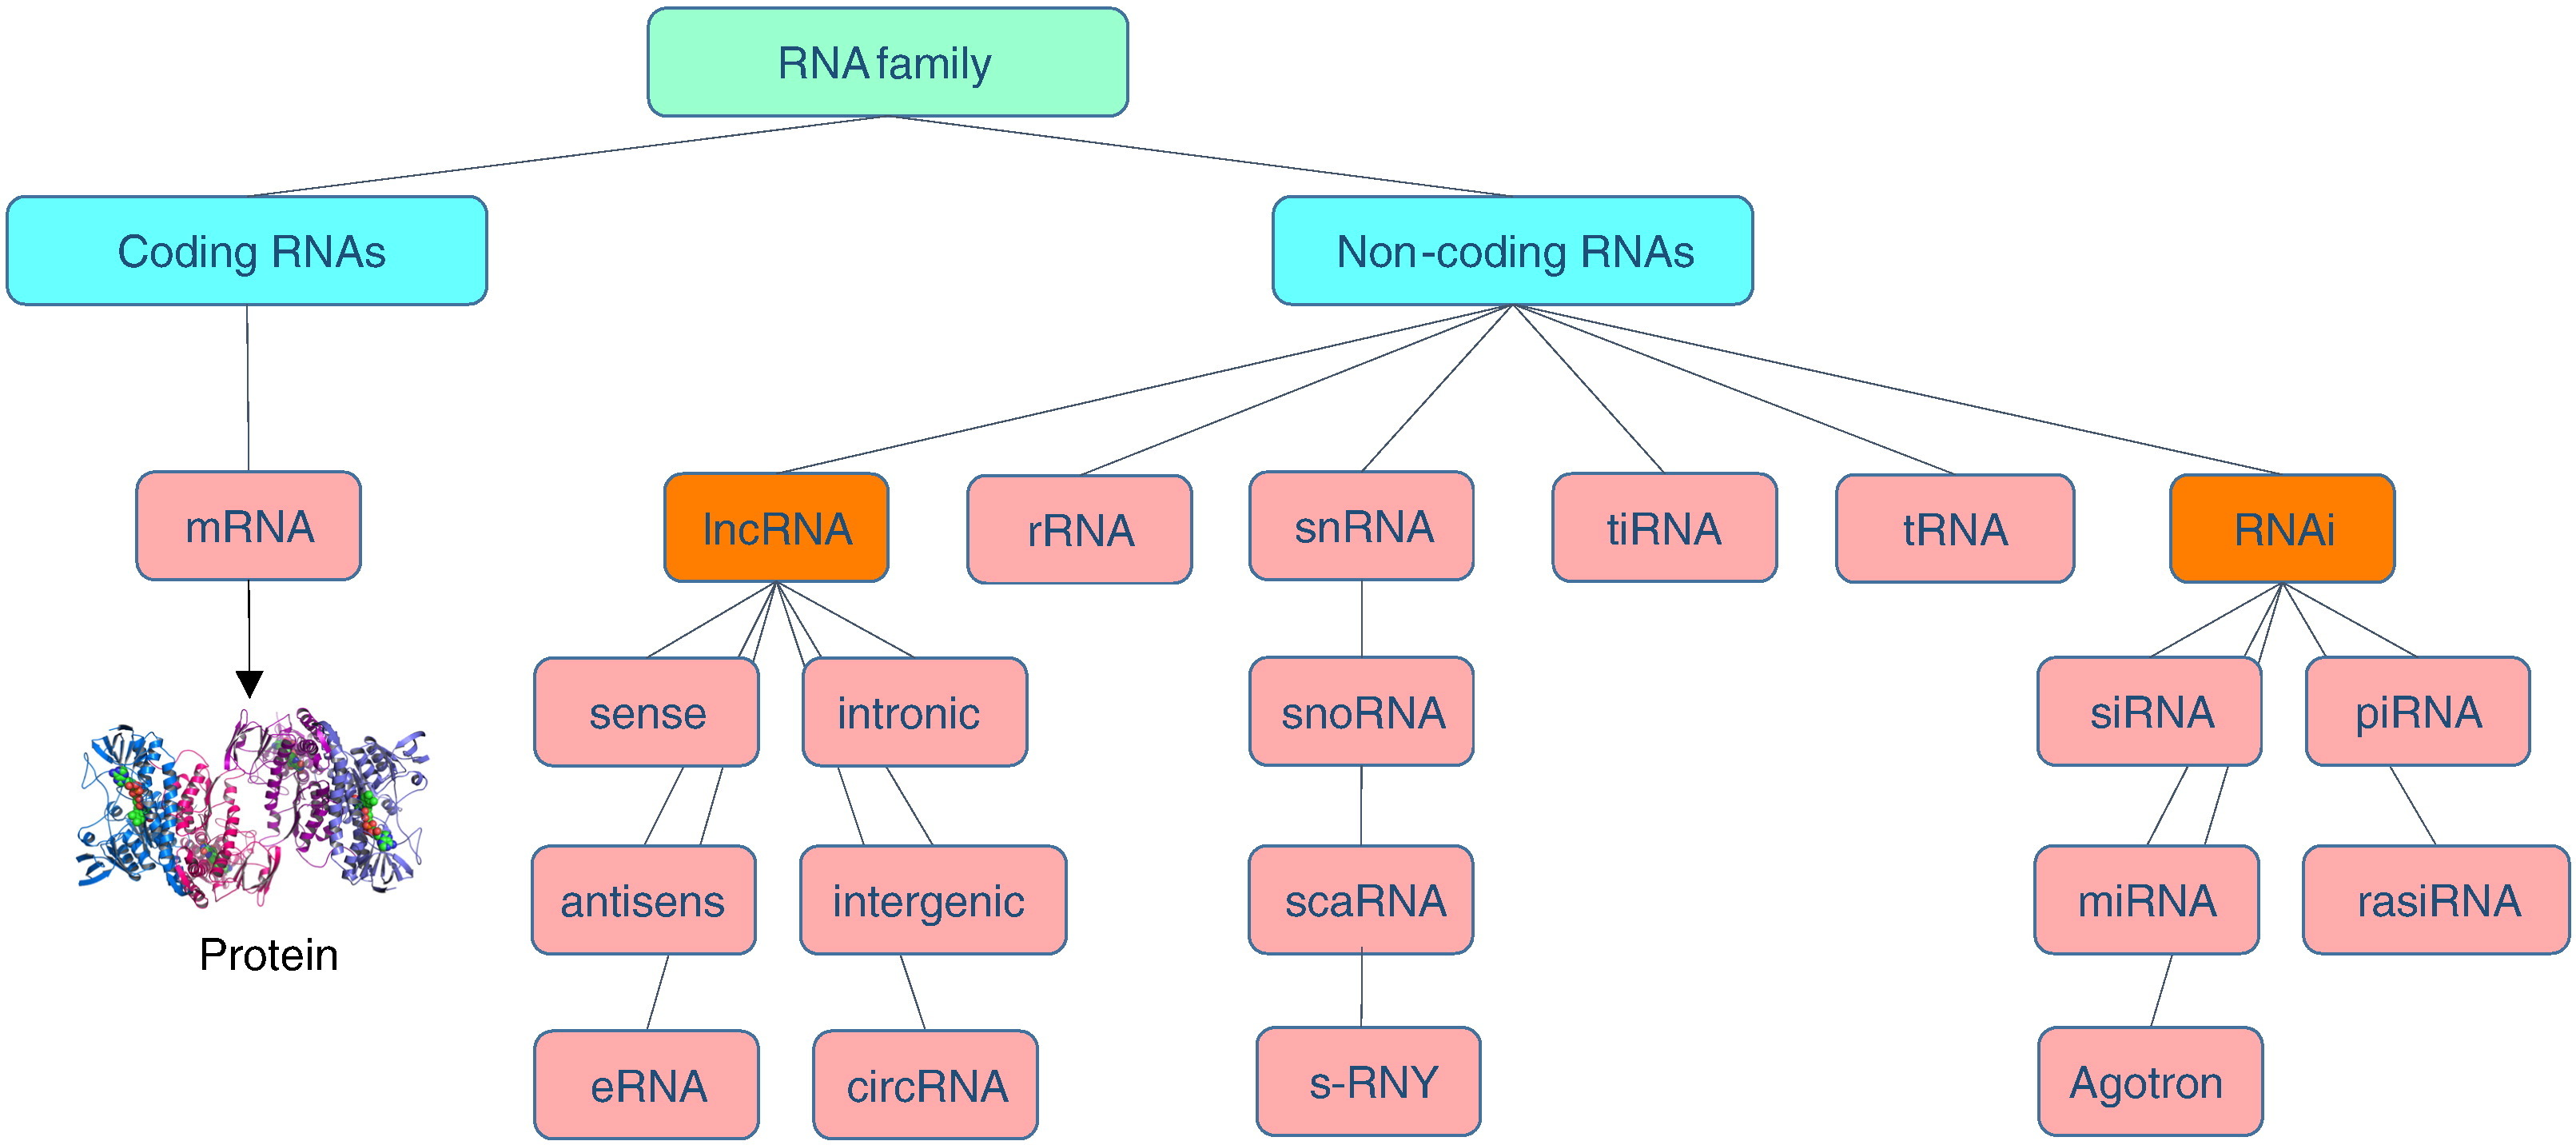
\includegraphics{img/intro/rna_familly_tree.jpg}

%% TRANSITION : parler des erreurs/variabilité biologique ? 

% \subsection{L'étude des perturbation du vivant pour la résolution de conditions cliniques}
\subsection{L'étude des perturbation de l'expression pour la résolution de conditions cliniques}

\section{Les technologies de séquençage de l'expression des gènes}
%% TODO : merge avec 1.1 partie d'avant

%% Nb publi pour le ration de microarray / RNA seq de jeux de données ?


%% historique des techno et qques specificités : https://journals.plos.org/ploscompbiol/article?id=10.1371/journal.pcbi.1005457
\begin{itemize}
\item Avant propos sur le développement des technologies de séquençage avec la quantification d'ARNm par rt-qPCR, le séquençage par gel, etc.
\item Transition vers les technologies de séquençage nouvelle génération
\end{itemize}

%% Un TRES bon site sur les technos de sequencage : http://education.knoweng.org/sequenceng/

\subsection{Microarray}
\begin{itemize}
\item Principe
\item Utilisation avec des exemple
\item Propriétés mathématiques et techniques
\begin{itemize}
    \item Distribution
    "Données continues, il est possible de construire des modèles d’analyse statistique ense basant sur des hypothèses de normalité des données (Smyth, 2004). Ces techniquesd’analyse, adaptées aux données gaussiennes ne peuvent pas être appliquées directementaux données RNA-seq qui sont des données de comptage, discrètes et positives" %% https://tel.archives-ouvertes.fr/tel-01424124/document
    \item Normalisation : Normalization is a process designed to identify and correct
technical biases. 2 types of norm : Between and within normalization (cf. formation marie laure meme si c'est pour le RNA-seq). Pourquoi normalisation log2 : le log pour passer à une échelle symétrique autour de 0, le 2 car c'est + facile à interpréter, chaque fois qu'on augmente le ratio Ti de 1, on double la up regulation  %%(https://www.researchgate.net/post/Why_do_we_usually_use_Log2_when_normalizing_the_expression_of_genes et https://www.nature.com/articles/ng1032z)
    \item Contrôle qualité
    \item Filtration
\end{itemize}
\item Explication du déclin mais avec contraste sur son utilité quand pas besoin de whole transcriptome
\end{itemize}

\subsection{RNA-Seq}
\begin{itemize}
\item Principe
\item Un mot sur le fait qu'on applique pas les mêmes méthodes de normalisation car la nature du signal n'est pas le même : une fluorescence pour le microarray (variable continue), et un comptage dans le cas du RNA-seq (variable discrète).
\item Explication de l'essor du RNA-seq (couts, precision, etc.)
\item Propriétés mathématiques : distribution(binomiale negative) %% Justification binomiale negative "Negative binomial (NB) distribution is the established gold standard, because of its ability to accurately model RNA-seq data with a low number of available replicates [7]." https://doi.org/10.1093/bib/bbx115
\item normalisations : %% cf. formation marie laure, il y a toutes les refs de publi a prendre
%% La raison du l'utilisation des pseudo counts et du log dans le RNA-seqyo : https://www.biorxiv.org/content/biorxiv/early/2020/05/19/2020.05.19.100214.full.pdf
\begin{itemize}
    \item Within sample
    \item Between samples
\end{itemize}
%% À classer entre within/between plus ahut selon ce qui est marqué dans la formation de marie laure : taille de librairie (= profondeur de sequencage), contenu en GC, taille des gènes, composition de la population d'ARN de chaque condition), contrôle qualité, filtration  (https://www.biostars.org/p/349881/)
\end{itemize}


%%%%%%%%%%%%%% LE TRAITEMENT STATISTIQUE DE L'INFORMATION BIOLOGIQUE %%%%%%%%%%%%%%


\section{Le traitement statistique de l'information biologique}
\subsection{L'expression différentielle : les acteurs majeurs}
\begin{itemize}
  \item Méthode de capture des acteurs majeurs
  \item Pas d'étude du système 
% \item Des statistiques descriptives à l'expression différentielle %% Bof, j'ai pas retrouvé de stade "stats explo" 
\end{itemize}

\subsection{La modélisation du vivant : des acteurs au système}
\begin{itemize}
\item De la régulation des gènes à son approximation par des modèles statistiques, en passant par la biologie des systemes qui est trop couteuse pour des organismes complexes %% mal formulé car dans le desordre (le dernier point devrait venir en 2e)
\item Transistion vers la modélisation par encodage de l'information dans des réseaux qui sont en fait des graph et qui sont moins couteux car probabilistes (ils ne sont pas la vérité mais une approximation)
\end{itemize}

\subsection{Les réseaux biologiques : le système vu via la théorie des graphes}
\begin{itemize}
\item Principe : les graphes sont une méthode de plus en plus utilisée dans la représentation du fonctionnement d'organismes puisqu'ils permettent d'avoir une vision à l'échelle du système tout entier.
%% Jolie intro à s'inspire : https://www.nature.com/articles/s41467-019-08746-5
\item Différences / ressemblance entre graphe et reseau ?
\item Les types de réseaux/graphes rencontrés en biologie et plus particulièrement en expression des gènes : small-world
\item Les problèmes de visualisation de grands réseaux %% section layout de ce livre https://sites.fas.harvard.edu/~airoldi/pub/books/BookDraft-CsardiNepuszAiroldi2016.pdf
\end{itemize}


%%%%%%%%%%%%%%%%%% LES RESEAUX DE CO-EXPRESSION %%%%%%%%%%%%%%%%%%


\section{Les réseaux de  co-expression}

%% GROOOOOSSSE PUBLI REVIEW sur la co-expression ET la comparaison de modules, aka co-expr differentielle https://doi.org/10.1109/TCBB.2019.2893170

\subsection{But}
"Gene co-expression networks seek to identify transcrip- tional patterns indicative of functional interactions and regulatory relationships between genes" %%https://genomebiology.biomedcentral.com/articles/10.1186/s13059-019-1700-9 + Barabási A-L, Gulbahce N, Loscalzo J. Network medicine: a network-based approach to human disease. Nat Rev Genet. 2011;12:56–68. + Furlong LI. Human diseases through the lens of network biology. Trends Genet. 2013;29:150–9.

\subsection{Principe}
%% Relire `van Dam, S., Võsa, U., van der Graaf, A., Franke, L. & de Magalhães, J. P. Gene co-expression analysis for functional classification and gene–disease predictions. Brief. Bioinform. bbw139 (2017). doi:10.1093/bib/bbw139`
\begin{itemize}
    \item Réseaux binaires (0 = pas de connexion, 1 = connexion). Pour et contres.
    \item Réseaux pondérés. Pourquoi c'est vers ça qu'on s'est orientés ? Car les connections entre gènes ne sont pas binaires, elles sont plutot multiples et très dépendantes temporellement. Une meme cellule échantillonnée à des temps différents aura un profil plus ou moins différent. On y retrouvera les grandes fonctions clefs mais les aspects plus variables auront peut etre changé. D'où aussi la nécessité d'un bon nombre d'échantillons pour assurer la validité des résultats. Sinon les correlations ne sont pas représentatives.
\end{itemize}
\subsection{Construction}
\begin{itemize}
\item Les différents scores de similarité : Pearson, Spearman, bicor, mutual information
\item La pondération des scores (adjacence et TOM) et la propriété d'invariance d'échelle (scale-free). Reparler de barbarasi et son celebre article (https://science.sciencemag.org/content/325/5939/412/tab-pdf) + Pourquoi elle est parfois encore discutée (https://www.nature.com/articles/s41467-019-08746-5) alors que tout de même pertinente en biologie. 
\end{itemize}
\subsection{Détection de modules}
\begin{itemize}
    \item Notion de communauté
    \item Définition du partitionnement (clustering) et des différentes techniques
\end{itemize}

\subsection{Exploitation des modules de gènes}

\subsubsection{Intégration biologique}
%% AKA knowledge driven
\begin{itemize}
    \item Enrichissement
    \item Test d'association
\end{itemize}

\subsubsection{Association phenotypique}
%% aussi knowledge driven

%%\subsection{Capitalisation sur l'information intrinsèque aux données}

\subsubsection{Étude topologique}
%% AKA data driven

%% Note : à voir si je présente aussi ici la comparaison de module vu que je vais ptet évoquer l'expression differentielle ici pour faire le parallele avec l'analyse transcripto classique. Sinon ça ira dans l'intro du chapitre avec l'article de GWENA.

\begin{itemize}
    \item Degré
    \item Définition de hub gene
    A trier / ordonner entre les différentes définitions, ce qu'elles visent, ce qu'elles appaortent et si possible une comparaison d'entre elles. On distinguera les mesure purement basées sur la theorie des graphs et celles impliquant des mesures statistique de significativité d'un gene comme hub (cf publi sur DHGA)
    \begin{itemize}
        \item Def 1 : Network theory : "A node is defined as hub node, if its connection degree is greater than average connection degree of the network" %% https://www.ncbi.nlm.nih.gov/pmc/articles/PMC5215982/
        \item Def 2 : Network hubs, the core elements in the network, can be defined using a range of different measures. These measures quantify distinct aspects of topological centrality, which can be defined as the capacity of a node to influence or be influenced by other nodes by virtue of its connection topology (Fornito et al., 2016).
    \end{itemize}
\end{itemize}
\subsubsection{Expression différentielle}
Pas sur de foutre ca là... Peut etre plutot en intro de la section complete en guise de "En analyse RNA classique, une méthode data driven est l'expression différentielle, mais en co-expression on a a disposition plus d'information extractable, et ce grace a la theorie des graphes" 

\subsubsection{Comparaison de modules}

Ou co-expression différentielle
%% "However, searching for differences in networks requires great sensitivity to the initial choice of data. For example, the absence of a shared link in mouse and human co-expression networks does not necessarily indicate divergent function. Instead, differences in the mouse and human co-expression networks may indicate differences in the technical platforms or the experimental conditions used to build the networks" http://doi.org/10.1371/journal.pgen.1000776

\subsection{Interprétation des résultats}

\subsubsection{Comparabilité des résultats issus de RNA-seq et de microarray}
\begin{itemize}
    \item Pas les meme hub genes %% "Microarray and RNA-seq-derived networks have different hub genes" https://academic.oup.com/bioinformatics/article/31/13/2123/196230
\end{itemize}


%%%%%%% L'INTÉRÊT DE l'ANALYSE PAR CO-EXPRESSION POUR L'ÉTUDE DU VIEILLISSEMENT %%%%%%%


\section{Le vieillissement, système hautement imbriqué}
%% Idée de début de paragraphe
S'il est une condition biologique où les réseaux de co-expression sont particulièrement bien adpatés, c'est bien le vieillissement. Source multi-factorielle de changements dans l'organisme, il est chez l'humain à l'origine d'une dégradation progressive des fonctions de base du corps.

\subsection{Définition biologique}
\begin{itemize}
    \item Facteurs : raccourcissement des télomères, phénomènes d'inflammation, réduction de la machinerie cellulaire
    \item Manifestation : Ralentissement de la division cellulaire, développement de cellules non-fonctionnelles / nocives (aka tumeurs), malfonctionnement des tissus/organes
\end{itemize}

\subsection{Enjeux}
Un enjeu de santé publique
\begin{itemize}
    \item Susceptibilité aux maladies opportunistes
    \item tdeetAutonomie patient
    \item Médicalisation précoce
\end{itemize}

\subsection{La capture de l'information liée au vieillissement par la transcriptomique}

\begin{itemize}
    \item La dérégulation de la transcription comme phénomène précédemment mentionné
    \item L'insuffisance de la capture de biomarqueurs pour un processus aussi compliqué que le vieillissement. Donc la nécessité d'une étude en réseau
    \item 
    
\end{itemize}
%% https://doi.org/10.1007/978-981-32-9005-1_3


\section*{Phrases utiles à retravailler et intégrer}

\begin{itemize}
\item "Studies have shown that each gene is estimated on average to interact with four to eight other genes1 and to be involved in 10 biological functions" [10.1038/s41598-017-18705-z]
\item "A very clear partition of different biological networks is provided by Christensen et al. [1], who separated these networks into five main categories as follows: [metabolic networks, signal transduction networks,transcriptional regulatory networks, protein-protein networks, functional gene networks]" [10.1093/bfgp/elt003]
%% Bouquin à la coloc de Clément à Sète, pas retrouvé sur le net jusque là 
\item "Le vieillissement est un continuum conduisant une personne en bonne santé à une réduction de sa réserve fonctionnelle, puis de sa capacité fonctionnelle et de sa qualité de vie. CEs différents aspects ne décrivent pas un chemin linéaire ou ordonné." [Patient agé : particularités de la consultation, Gilles Berrut]
\item "It has been reported that nearly one in four studies uses public data to address a biological problem without generating new raw data (Rung and Brazma, 2013)." [10.3389/fpls.2016.00444]
\end{itemize}


%% Points que je veux aborder :
%%  - Definition des reseau arrete / noeud
%%  - Definition des modules par l'effet de modularité
%%  - Ce à quoi ils peuvent servir : raccrochage de fonction a certains genes, detection de pathways, detection de reseaux de regulation



%%    • Weighted aspect [trop general, aura plutot sa place dans la thèse]
%% But because of the multi-functionality aspect of each gene, such GCN using only binary state between genes (1 = correlated, 0 = not correlated) lead to information loss\cite{Langfelder2008}. Therefore, a new class of GCN have been developed: weighted gene co-expression networks. One of the most famous implementation is the R package WGCNA\cite{Langfelder2008}, but one can also mention the recent wTO\cite{Gysi2018} package which consider both positive and negative correlation for GCN building. Instead of a simple pairwise correlation, these packages weight the similarity score by calculating a factor taking into account other properties of the network. In the case of WGCNA, it specifies an adjacency score which raise the similarity to a power, which will increase the strength of strong similarities while keeping low week ones. In the case of wTO, it determine an average accounting for all common neighbors of a node.

%%    • Topological aspect
%%    • Co-expression properties (Scale-free-network entre autres ?)



%% Infos sur la peau : these super interessante => https://dumas.ccsd.cnrs.fr/dumas-01599807/document% \end{itemize}

          % introduction
\chapter{Titre du chapitre}     % numéroté

Texte du chapitre.



%% \bibliographystyle{unsrt}     % style de la bibliographie
%% \bibliography{}               % production de la bibliographie    % chapitre 1
\setcounter{chapter}{3}
\chapter*{Chapitre 2 - À définir}
\phantomsection\addcontentsline{toc}{chapter}{Chapitre 2 - À définir} 
%%\chapter{Titre du chapitre}     % numéroté

Idées :
\begin{itemize}
    \item Rajout d'information protéique pour "consolider" le réseau ?
    \item Rajout d'une méthode de réseau consensus à GWENA ?
    \item ???
\end{itemize}

\section{test bis}

\bibliographystyle{}              % style de la bibliographie
\bibliography{}                   % production de la bibliographie
    % chapitre 2, etc.
\chapter*{Conclusion}         % ne pas numéroter
\phantomsection\addcontentsline{toc}{chapter}{Conclusion} % dans TdM

Une thèse ou un mémoire devrait normalement se terminer par une
conclusion, placée avant les annexes, le cas échéant. Celle-ci est
traitée comme un chapitre normal, sauf qu'elle n'est pas numérotée.


% Publi utile pour les perspectives :
% https://onlinelibrary.wiley.com/doi/abs/10.1111/gbb.12106


Le vieillissement est un phénomène dont la complexité n'a d'égal que la multiplicité de ses manifestations. Tantôt origine, tantôt conséquence, les phénomènes de sa manifestations impactent de nombreux mécanismes cellulaire et moléculaires : sénescence et cellules souches, inflammation chronique de faible intensité, raccourcissement des télomères, etc. \cite{Lopez-Otin2013}. Pour distinguer de façon certaine chacun des altérations basales chez chaque individu, un nombre important d'échantillons est nécessaire. L'étude GTEx est à ce jour le plus gros regroupement de séquençage en terme d'individus/tissus non ciblé sur une pathologie. Sa réalisation permet d'étudier le vieillissement non plus dans ses manifestations les plus détaillées mais bien de rechercher les mécanismes communs à beaucoup des tissus composant le corps humain. Cependant            % conclusion

\appendix                       % annexes le cas échéant

\chapter{Titre de l'annexe}     % numérotée

Texte de l'annexe.
                % annexe A

\end{document}
